\chapter{Selection in protein coding {DNA} sequences}
\minitoc
\label{sec:selection}
The first chapter recalled the framework of molecular evolution, and how the evolutionary trajectory of sequences is defined in terms of mutation, selection and drift. 
This parametrization required a given selection coefficient associated to mutation, or required the fitness of each particular sequence to be defined.
However, this introduction remained so far elusive on the relationship between sequence and fitness.
This chapter, on the other hand, solely focus on the mapping from sequence to fitness, in the special case of protein coding \acrshort{DNA} sequence.
It will seek to clarify the relationship between protein sequence, protein thermodynamic, protein function, and organismal fitness, such as to derive the selective pressures shaping proteins coding \acrshort{DNA} sequences.
It is also important to emphasize whether they are general principles, or do this relationship between sequence and fitness depends on the specific protein, organism, and environment.

\section{Protein coding DNA sequences}

Proteins have a variety of molecular and cellular roles, they are the enzymes that catalyses chemical bonds, they regulate cell processes and control their rates, they carry signals within the cell and across membranes, they bind and transport small molecules, they form cellular structures, and so on.
This variety of roles is accomplished by a variety of three-dimensional shapes.
A protein's three-dimensional shape is in turn determined by the linear one-dimensional sequence of amino-acids.
Just as \acrshort{DNA} is oriented because of the asymetry of nucleotides, proteins are oriented due to asymetry of amino-acids, one end is called \gls{N-ter} and the other end C-terminus. 
In practice, proteins size can range from fewer than $20$ to more than $5000$ amino acids, although an average protein is about 350 amino acids long.
Although each of the 20 different amino acids has unique biochemical properties, they can be classified broadly into four categories.
Charged amino-acids can be either basic (positively charged) or acidic (negatively charged).
On the other hand, non charged amino-acids can however be polar due to an uneven charge distribution, such that they can form hydrogen bonds with water.
Consequently, polar amino acids are called hydrophilic, and are often found on the outer surface of folded proteins.
Also, non charged amino-acids can have a uniform charge distribution, and do not form hydrogen bonds with water.
Reciprocally, these non polar amino-acids are called hydrophobic and tend to be found in the core of folded proteins.

\subsection{Genetic code}

Because the $20$ letter alphabet of proteins is different to the $4$ letter alphabet of nucleic acid (DNA and RNA), there is not a one-to-one correspondence between the two alphabets.
Instead, amino acids are encoded by codons, a consecutive sequences of 3 nucleotides, yielding $4^3=64$ possible permutations, more than sufficient to encode the 20 different amino acids.
Moreover, three stop codons signals termination of the protein, such that 61 of the 64 codons are used to encode amino acids.
Biochemical translation from \gls{codon} to amino-acid mechanistically emanates from transfer \acrshort{RNA} (\acrshort{tRNA}).
More precisely, codons binds to \acrshort{tRNA} \acrshort{tRNA} trough an anticodon, three consecutive bases that are complementary and antiparallel to the associated \gls{codon}, using canonical Watson-Crick base pairing (A-T and G-C).
On the other end, \acrshort{tRNA} structure complexes uniquely with one the $20$ amino acid, where the catalytic reaction is performed by aminoacyl-tRNA synthetase.

However, there is not a one-to-one correspondence between codon and \acrshort{tRNA}, such that the number of tRNA in the cell is not exactly $61$.
On one hand, different tRNAs can carry the same anticodon but could display varying efficiency in translation, adding a layer of regulation to the process of protein synthesis.
On the other hand, some tRNA can pair with codons due to non standard pairing, due to geometrical relaxation.
More precisely, the first two bases in the codon bond strongly to the anticodon of the tRNA, while the third base can be subject to non standard pairing, only between U or G, the pairing is less specific and in fact two bases can be interchangeably recognized by the tRNA.
Due to the specificity inherent in the first two nucleotides of the codon, if one amino acid is coded for by multiple anticodons and those anticodons differ in either the second or third position (first or second position in the codon) then a different tRNA is required for that anticodon.
The minimum requirement to satisfy all possible $61$ codons is $31$ tRNAs for the amino acids and one initiation codon.
Altogether, \acrshort{tRNA} along with aminoacyl-tRNA synthetase constitute the machinery necessary for translating \gls{codon} into amino-acid, according the DNA genetic code given in table \ref{table:genetic_code}, which is used almost universally by all organisms.


\begin{table}[h]
	\resizebox{\columnwidth}{!}{%
		\begin{tabular}{|c|l|c|l|c|l|c|l|c|c|}
			\hline
			& \multicolumn{2}{c|}{T} & \multicolumn{2}{c|}{C} & \multicolumn{2}{c|}{A} & \multicolumn{2}{c|}{G} & \\ \hline \hline
			\multirow{4}{*}{T} & TTT & \cellcolor{Nonpolar} & TCT & \cellcolor{Polar} & TAT & \cellcolor{Polar} & TGT & \cellcolor{Polar} & T \\
			\cline{2-2} \cline{4-4} \cline{6-6} \cline{8-8} \cline{10-10}
			& TTC & \cellcolor{Nonpolar} \multirow{-2}{*}{Phenylalanine (Phe/P)} & TCC & \cellcolor{Polar} & TAC & \cellcolor{Polar} \multirow{-2}{*}{Tyrosine (Tyr/Y)} & TGC & \cellcolor{Polar} \multirow{-2}{*}{Cysteine (Cys/C)} & C \\
			\hhline{|~|-|-|-|>{\arrayrulecolor{Polar}}->{\arrayrulecolor{black}}|-|-|-|-|-|}
			& TTA & \cellcolor{Nonpolar} & TCA & \cellcolor{Polar} & TAA & \cellcolor{Stop} Stop (Ochre) & TGA & \cellcolor{Stop} Stop (Opal) & A \\
			\hhline{|~|-|>{\arrayrulecolor{Nonpolar}}->{\arrayrulecolor{black}}|-|>{\arrayrulecolor{Polar}}->{\arrayrulecolor{black}}|-|-|-|-|-|}
			& TTG & \cellcolor{Nonpolar} & TCG & \cellcolor{Polar} \multirow{-4}{*}{Serine (Ser/S)} & TAG & \cellcolor{Stop} Stop (Amber) & TGG & \cellcolor{Nonpolar} Tryptophan (Trp/W) & G \\
			\hhline{|-|-|>{\arrayrulecolor{Nonpolar}}->{\arrayrulecolor{black}}|-|-|-|-|-|-|-|}
			\multirow{4}{*}{C} & CTT & \cellcolor{Nonpolar} & CCT & \cellcolor{Nonpolar} & CAT & \cellcolor{Basic} & CGT & \cellcolor{Basic} & T \\
			\cline{2-2} \cline{4-4} \cline{6-6} \cline{8-8} \cline{10-10}
			& CTC & \cellcolor{Nonpolar} & CCC & \cellcolor{Nonpolar} & CAC & \cellcolor{Basic} \multirow{-2}{*}{Histidine (His/H)} & CGC & \cellcolor{Basic} & C \\
			\hhline{|~|-|>{\arrayrulecolor{Nonpolar}}->{\arrayrulecolor{black}}|-|>{\arrayrulecolor{Nonpolar}}->{\arrayrulecolor{black}}|-|-|-|>{\arrayrulecolor{Basic}}->{\arrayrulecolor{black}}|-|}
			& CTA & \cellcolor{Nonpolar} & CCA & \cellcolor{Nonpolar} & CAA & \cellcolor{Polar} & CGA & \cellcolor{Basic} & A \\
			\cline{2-2} \cline{4-4} \cline{6-6} \cline{8-8} \cline{10-10}
			& CTG & \cellcolor{Nonpolar} \multirow{-6}{*}{Leucine (Leu/L)} & CCG & \cellcolor{Nonpolar} \multirow{-4}{*}{Proline (Pro/P)} & CAG & \cellcolor{Polar} \multirow{-2}{*}{Glutamine (Gln/Q)} & CGG & \cellcolor{Basic} \multirow{-4}{*}{Arginine (Arg/R)} & G \\
			\hline
			\multirow{4}{*}{A} & ATT & \cellcolor{Nonpolar} & ACT & \cellcolor{Polar} & AAT & \cellcolor{Polar} & AGT & \cellcolor{Polar} & T \\
			\cline{2-2} \cline{4-4}\cline{6-6} \cline{8-8} \cline{10-10}
			& ATC & \cellcolor{Nonpolar} & ACC & \cellcolor{Polar} & AAC & \cellcolor{Polar} \multirow{-2}{*}{Asparagine (Asn/N)} & AGC & \cellcolor{Polar} \multirow{-2}{*}{Serine (Ser/S)} & C \\
			\hhline{|~|-|>{\arrayrulecolor{Nonpolar}}->{\arrayrulecolor{black}}|-|>{\arrayrulecolor{Polar}}->{\arrayrulecolor{black}}|-|-|-|-|-|}
			& ATA & \cellcolor{Nonpolar} \multirow{-3}{*}{Isoleucine (Ile/I)} & ACA & \cellcolor{Polar} & AAA & \cellcolor{Basic} & AGA & \cellcolor{Basic} & A \\
			\hhline{|~|-|-|-|>{\arrayrulecolor{Polar}}->{\arrayrulecolor{black}}|-|>{\arrayrulecolor{Basic}}->{\arrayrulecolor{black}}|-|>{\arrayrulecolor{Basic}}->{\arrayrulecolor{black}}|-|}
			& ATG & \cellcolor{Nonpolar} Methionine (Met/M) & ACG & \cellcolor{Polar} \multirow{-4}{*}{Threonine (Thr/T)} & AAG & \cellcolor{Basic} \multirow{-2}{*}{Lysine (Lys/K)} & AGG & \cellcolor{Basic} \multirow{-2}{*}{Arginine (Arg/R)} & G \\
			\hline
			\multirow{4}{*}{G} & GTT & \cellcolor{Nonpolar} & GCT & \cellcolor{Nonpolar} & GAT & \cellcolor{Acidic} & GGT & \cellcolor{Nonpolar} & T \\
			\cline{2-2} \cline{4-4} \cline{6-6} \cline{8-8} \cline{10-10}
			& GTC & \cellcolor{Nonpolar} & GCC & \cellcolor{Nonpolar} & GAC & \cellcolor{Acidic} \multirow{-2}{*}{Aspartic acid (Asp/D)} & GGC & \cellcolor{Nonpolar} & C \\
			\hhline{|~|-|>{\arrayrulecolor{Nonpolar}}->{\arrayrulecolor{black}}|-|>{\arrayrulecolor{Nonpolar}}->{\arrayrulecolor{black}}|-|-|-|>{\arrayrulecolor{Nonpolar}}->{\arrayrulecolor{black}}|-|}
			& GTA & \cellcolor{Nonpolar} & GCA & \cellcolor{Nonpolar} & GAA & \cellcolor{Acidic} & GGA & \cellcolor{Nonpolar} & A \\
			\cline{2-2} \cline{4-4} \cline{6-6} \cline{8-8} \cline{10-10}
			& GTG & \cellcolor{Nonpolar} \multirow{-4}{*}{Valine (Val/V)} & GCG & \cellcolor{Nonpolar} \multirow{-4}{*}{Alanine (Ala/A)} & GAG & \cellcolor{Acidic} \multirow{-2}{*}{Glutamic acid (Glu/E)} & GGG & \cellcolor{Nonpolar} \multirow{-4}{*}{Glycine (Gly/G)} & G \\
			\hline
	\end{tabular}}
	\caption[The Genetic Code]{
		The genetic code DNA table translating codons into amino-acids.
		Amino-acids are represent into $4$ categories based on the electrochemical properties.
		Non-polar in yellow (\textcolor{Nonpolar}{\ding{110}}), polar in green (\textcolor{Polar}{\ding{110}}), basic in blue (\textcolor{Basic}{\ding{110}}) and finally acidic in red (\textcolor{Acidic}{\ding{110}}).
		Stop codons are represented in black (\textcolor{Stop}{\ding{110}}).
		The synonymous codons encoding for the same amino-acid are usually different by their third codon position, the wooble base. 
	}
	\label{table:genetic_code}
\end{table}

Since there are 61 coding codons and only 20 amino acids, there is a necessary redundancy in the code.
Thus, amino acids \footnote{With the notable exception of methionine and tryptophan} are encoded by synonymous codons, which are interchangeable in the sense of producing the same amino acid.
Because mutation are at the nucleotide level and effect only one base, any codon can have at most $9$ possible transitions to another codons (see figure \ref{fig:graph-codons-aa}, right panel).
Moreover, it is possible that some pairs of amino-acids are not accessible through a single non-synonymous transition between the underlying codons (see figure \ref{fig:graph-codons-aa}, right panel), such that if for example these two amino-acids are high fitness, they would need to pass trough a fitness valley. 

\begin{figure}[htb!]
	\begin{center}
		\begin{minipage}{0.48\linewidth}
			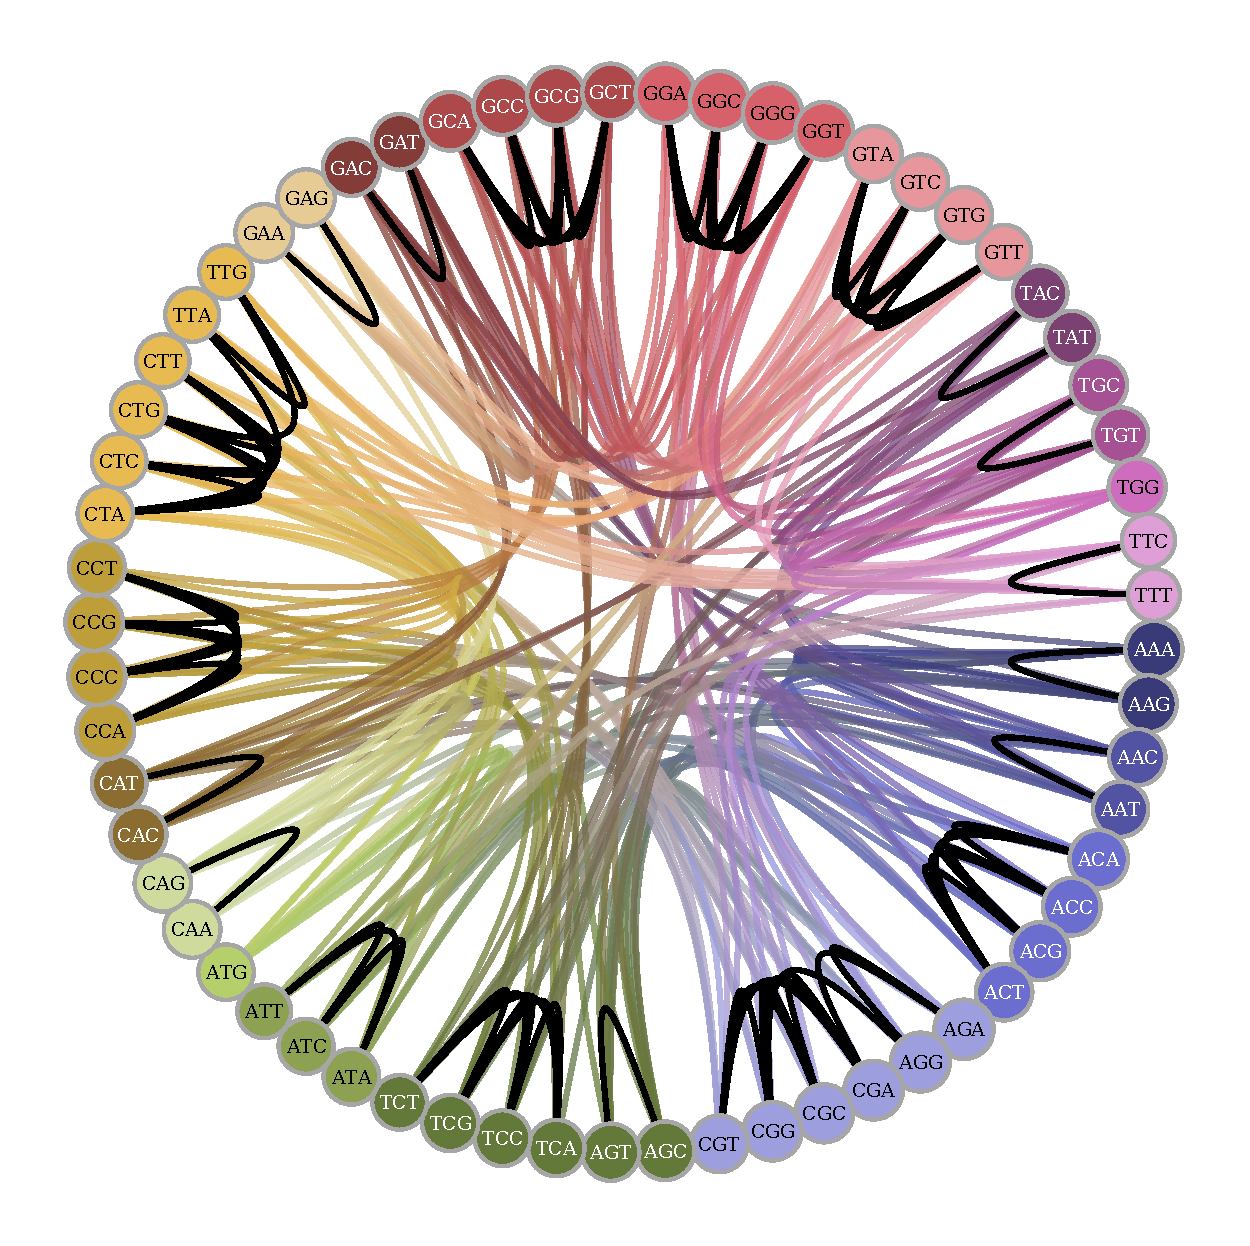
\includegraphics[width=\linewidth, page=1]{figures/gt-codon-tab20b.pdf}
		\end{minipage}%
		\hfill
		\begin{minipage}{0.49\linewidth}
			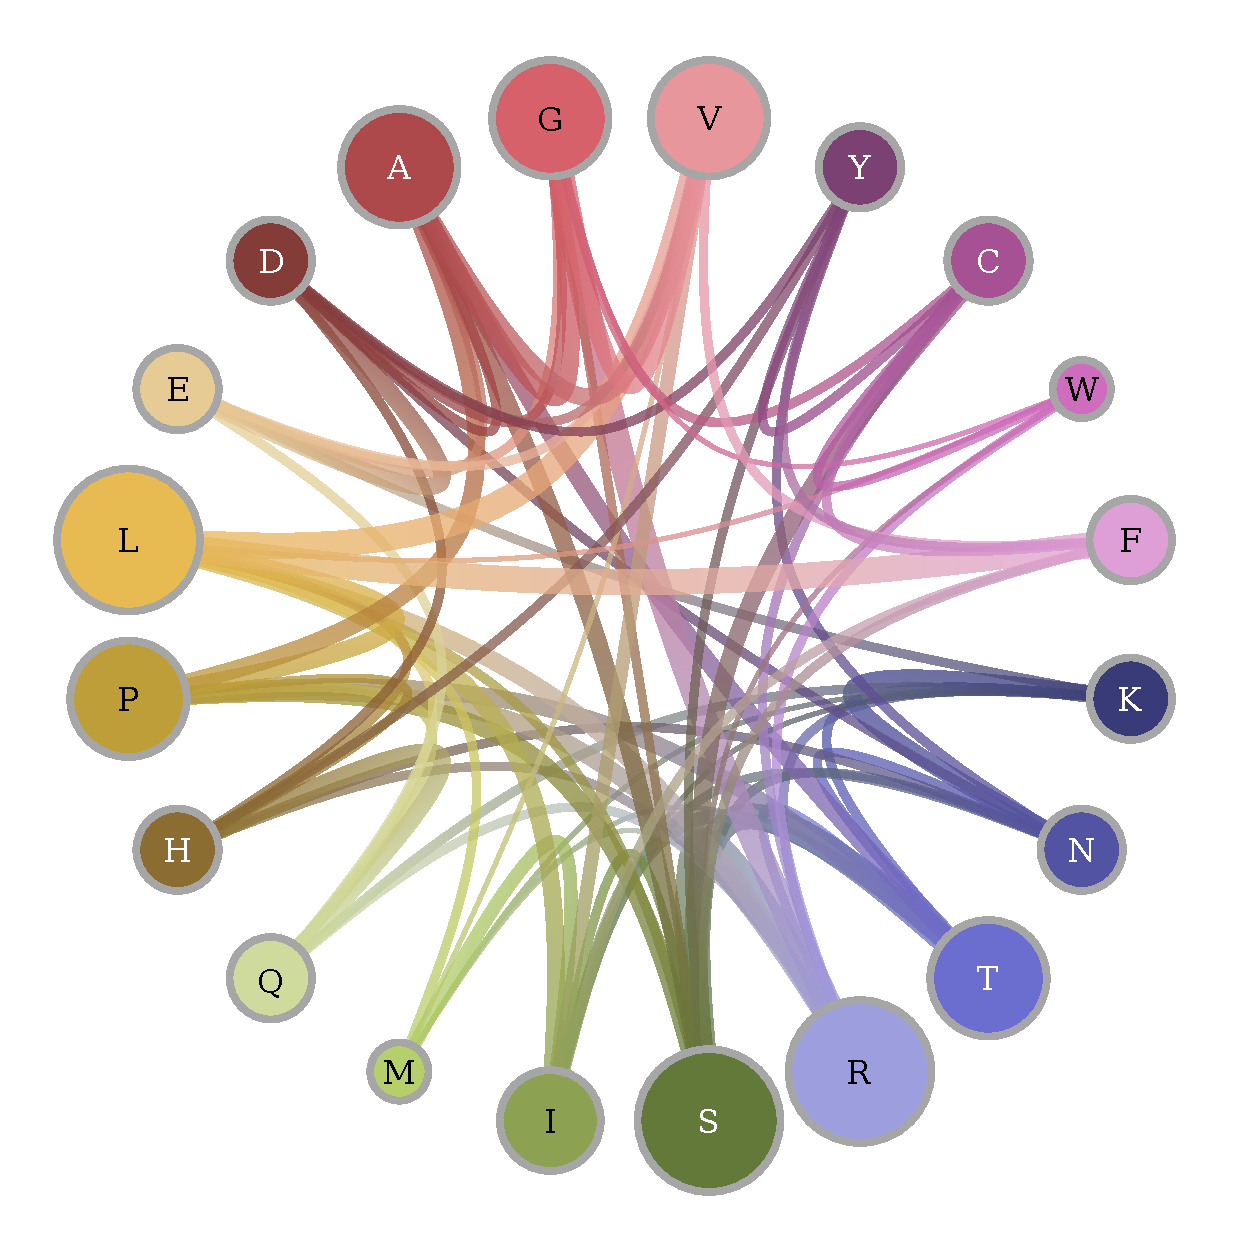
\includegraphics[width=\linewidth, page=1]{figures/gt-aa-tab20b.pdf}
		\end{minipage}
	\end{center}
	\caption[Graphs of codon and amino-acid transitions]{
		\label{fig:graph-codons-aa}
		Graphs of possible one nucleotide transition between codon (left panel) and between amino-acid (right panel).
		Nodes corresponds to codons (left panel) and amino-acid (right panel), and node's color represent the encoded amino-acid.
		Additionanly, for amino-acids the size of nodes represent the number of underlying codons.
		An edge between two codons corresponds to a one nucleotide transition, such that a codon can have at most $9$ possible transitions. 
		Similarly, en edge between two amino-acids correspond to a one nucleotide non-synonymous transition between the underlying codons, and the weight of the edges represent the number such possible transitions.
		Non-synonymous transition are represented in colored gradient, while synonymous transitions are depicted in black.
		The graph of the $61$ codons contains $263$ transitions, $67$ of them are syonymous while $196$ are non-synonymous.
		The radius of the graph is three, such that the most distant amino-acids are at most three transition away.
		Codons encoding for the same amino-acid are all fully connected by synonymous changes, expect for Serine where a transition for (TCT, TCG, TCC,	TCA) to (AGT, AGC) requires passing trought another amino-acid, hence a least two non-synonymous transitions.
		From the perspective of amino-acids, the graph of the $20$ amino-acids contains $75$ non-synonymous transitions. 
		The graph is not fully connected and do not form a clique, and the radius of the graph is also three, because a transition from Methione to Tyrosine requires at least three non-synonymous transitions. 
		Altogether, for all the possible $190$ pairs of amino-acids, $114$ pairs requires at least two non-synonymous transitions, and one pair (M-Y) requires at least three non-synonymous transitions.
	}
\end{figure}
\subsection{Codon substitution models}
Studying evolution of protein coding \acrshort{DNA} sequences at the nucleotide level, while disregarding the biochemical properties of amino-acids is a major shortcoming not taking into account.
Conversely, studying the evolutionary history of the protein instead of the \acrshort{DNA} sequence, meaning translating nucleotide sequences into amino-acid sequences, and designing models at the amino-acid level also has the major shortcoming of not taking into account that the mutation process occurs at the nucleotide level.
These shortcomings are both addressed by \gls{codon} models, where the complexity of the genetic code is seen as an asset rather than an encumbrance.
Indeed the redundancy in the genetic code can be leveraged to disentangle mutation and selection in protein coding \acrshort{DNA} sequences, under the approximation that selection occurs at the protein level in first approximation, while the mutation process occurs at the \acrshort{DNA} level.
The genetic code allows to split mutations into \gls{neutral} and selected mutations, where synonymous mutattion is deemed neutral, meaning not changing the translated amino-acid, or non-synonymous, meaning the translated amino-acid will be different.
The degeneracy of the genetic code is thus an advantage when one devises a model at the \gls{codon} level in \acrshort{DNA} sequences.

The mutation rate from \gls{codon} $\ci$ to $\cj$ depends on the underlying nucleotide change between the \gls{codon}, if $\ci$ to $\cj$ are only a mutation away, $\nucitoj$ denotes the nucleotide change between the codons. The \gls{codon} mutation rate is then given by the mutation matrix ${\mutmatrix_{\nucitoj}}$. Altogether, the mutation rate from \gls{codon} $\ci$ to $\cj$ is:
\begin{equation}
\begin{dcases}
\mu_{\itoj} & = 0 \text{if $\ci$ and $\cj$ are one mutation away,} \\
\mu_{\itoj} & = \mu \mutmatrix_{\nucitoj} \text{ else }
\end{dcases}
\end{equation}

\begin{equation}
\label{eq:mutrates}
\Mutmatrix = \begin{pmatrix}
- & {\exchan_{AC} \mutequi_C} & {\exchan_{AG}\mutequi_G} & {\exchan_{AT}\mutequi_T} \\ 
{\exchan_{AC}\mutequi_A} & - & {\exchan_{CG}\mutequi_G} & {\exchan_{CT}\mutequi_T} \\ 
{\exchan_{AG}\mutequi_A} & {\exchan_{CG}\mutequi_C} & - & {\exchan_{GT}\mutequi_T} \\ 
{\exchan_{AT}\mutequi_A} & {\exchan_{CT}\mutequi_C} & {\exchan_{GT}\mutequi_G} & - 
\end{pmatrix},
\end{equation}

The phylogeny-based method models the \gls{substitution} rate at the \gls{codon} level. Synonymous and non-synonymous mutations are treated differently. The rate of non-synonymous substitutions over the rate of synonymous substitutions (denoted $\omega=d_N/d_S$) is estimated as a parameter of the model \citep{Muse1994,Goldman1994}. Assuming synonymous mutations are \gls{neutral}, an $\omega>1$ signals an excess in the rate of non-synonymous substitutions, indicating that the protein is under adaptive evolution. Conversely, a default of non-synonymous substitutions, leading to $\omega<1$, means the protein is under purifying selection. However, in practice, protein are typically under a mix of adaptation and purifying selection, thus typically leading to an $\omega<1$ even in the presence of positive selection. More sophisticated methods have been proposed. In particular, site-models trying to detect specific site of the sequence with an $\omega>1$, have been developed \citep{Yang2001, kosiol_patterns_2008}.


In the case of synonymous mutations ($\cj \in \NiSyn $), the probability of fixation is independent of the original and target \gls{codon}, and equal $1/2 \Ne$. Finally ${\submatrix_{\itoj}}$ simplifies to: 
\begin{equation}
\submatrix_{\itoj} = \mu \mutmatrix_{\nucitoj}
\end{equation}
In the case of non-synonymous mutations ($\cj \in \NiNonSyn $), the probability of fixation depends on the difference of fitness between the amino-acid encoded by the codons:
\begin{align}
\submatrix_{\itoj} & = \omega \mu \mutmatrix_{\nucitoj}
\end{align}
Altogether, the $61$-by-$61$ codon substitution matrix is defined entirely by the mutation matrix and 
\begin{equation}
\begin{dcases}
\submatrix_{\itoj} & = 0 \text{ if $\ci$ and $\cj$ are non neighbors} \\
\submatrix_{\itoj} & = \mu_{\itoj} \text{ if $\ci$ and $\cj$ are syonymous} \\
\submatrix_{\itoj} & = \mu_{\itoj} \dfrac{4 \Ne \left({\fitj - \fiti}\right)}{{1 - \e^{4 \Ne \left({\fiti - \fitj}\right)} }} \text{ if $\ci$ and $\cj$ are non-syonymous} \\
\submatrix_{\ci, \ci} & = - \sum_{\cj \neq \ci} \submatrix_{\itoj}
\end{dcases}
\label{eq:codon-models}
\end{equation}
where the mutation rate between codon $\ci$ and $\cj$ is given by:
\begin{equation}
\begin{dcases}
\mu_{\itoj} & = 0 \text{ if } \cj \notin \Ni \\
\mu_{\itoj} & = \mu \mutmatrix_{\nucitoj} \text{ if } \cj \in \Ni
\end{dcases}
\end{equation}
One can identify the interplay between mutations acting at the \acrshort{DNA} level, and positive or negative selection acting at the protein level.
Thus, \gls{codon} \gls{substitution} models are crucial for a better modeling of the underlying evolution of protein-coding \acrshort{DNA} sequences, and consequently allow a better reconstruction of mutation, selection and demography.

\section{Insight from empirical data}

This section review the empirical evidence available, which will be important to keep in mind when the different models of selection will be 

Classical \gls{codon} models estimate a parameter $\dnds$, namely the ratio of the non-synonymous over the \gls{synonymous} rates \citep{Muse1994,Goldman1994}. In the so-called site-models, $\dnds$ is allowed to vary across sites, either via a finite mixture \citep{Yang2001}, an infinite mixture \citep{Huelsenbeck2006}, or as random effects from a parametric distribution \citep{lartillot_phylobayes_2013}. 
The fact that is far lower than 1 express the fact that proteins are mostly under a regime of purifying selection.

\subsection{Substitution rate across genes}

However, even for those proteins of comparable expression levels, their ERs still span several orders of magni- tude (Drummond and Wilke, 2008). Abundance likewise cannot account for the quasi log-normal distribution of the ER among genes in a genome, a fact observed from bacteria, yeast, worm, fly, mouse, and humans (Lobkovsky et al., 2010). These observations suggest that abundance, although a major deter- minant of ER, is not its only causal variable.
Lobkovsky, A.E., Wolf, Y.I., and Koonin, E.V. (2010). Universal distribution of protein evolution rates as a consequence of protein folding physics. Proc. Natl. Acad. Sci. USA 107, 2983–2988

The increased availability of genomic data for species across the tree of life prompted an extensive search for the major determinants of the protein \gls{substitution} rate. Surprisingly, the functional importance of a protein, widely thought to approximate the level of functional constraint, has only a minor role, whereas protein expression level is found to be a major determinant9 \citep{Zhang2015}

Because of the strong correlation between mRNA and protein concentrations, the negative correlation between protein concentration and evolutionary rate is also strong.
Drummond et al. showed that the correlation with \gls{substitution} rate is weaker for protein concentration than for mRNA concentration.
However, it is unclear whether this disparity is genuine or whether it simply reflects different qualities of proteomic and transcriptomic data.

\subsection{Substitution rate across sites}
It is well known that amino acid residues located inside a protein structure (that is, core residues) have more central roles than surface residues in protein folding stability.
However, surface residues show an E–R anticorrelation as strong as that of core residues, suggesting that selective pressures other than misfolding avoidance might also be present, especially on surface residues.

Yang et al. showed that the E–R anticorrelation is only moerately weakened by the removal of amino acids that stabilize protein folding and that the impact of this removal on the E–R anticorrelation is smaller when amino acids are removed from protein surfaces than from protein cores. 

linear relationship between evolutionary rate and RSA reflects a selection pressure on the amino acid level. \citep{Ramsey2011}

Causes of evolutionary rate variation among protein sites \citep{Echave2016}

The strength of selection is not typically homogeneous along the sequence.
For example, exposed sites are under lower selective pressure than buried sites \citep{Echave2016}.
In fact, selection differs in a way that depends on the local physico-chemical requirements \citep{Goldstein2016,Goldstein2017,Weber2019}.

Models must generally conform to observed properties of proteins, such as the observations that surface residues of globular proteins undergo \gls{substitution} more rapidly than those in the core,

In a recent work, we have shown that stability-constrained models that take into
account negative design for destabilizing misfolded conformations (Berezovsky, Zeldovich \& Shakhnovich, 2007; Noivirt-Brik, Horovitz \& Unger, 2009; Minning, Porto \& Bastolla, 2013) predict that both the \gls{substitution} rate and the entropy are maximal not at exposed sites with few contacts, as observed, but at sites where the number of contacts is intermediate, which can accomodate both hydrophobic and polar amino acids and are predicted to be extremaly tolerant to mutations (Jimenez, Arenas \& Bastolla, 2018). On the other hand, when stability with respect to misfolding is neglected, stability-constrained models predict that the variability is maximal at exposed sites with few contacts (Scherrer, Meyer \& Wilke, 2012; Echave, Jackson \& Wilke, 2015), but these kinds of models overestimate both the tolerance to mutations and the average hydrophobicity at almost all positions (Jimenez, Arenas \& Bastolla, 2018) and they score much worse than models that consider misfolding in \gls{likelihood} calculations (Arenas, Sanchez-Cobos \& Bastolla, 2015), so that models that consider misfolding have to be preferred. In contrast, structure-constrained models correctly predict that the variability is inversely related with the number of native contacts (Huang et al., 2014). These results support the view that the structural effect of mutations cannot be neglected, in particular at sites with intermediate numbers of contacts that are extremely tolerant to mutations under the point of view of the stability.

The evolutionary variability of a protein site is strongly influenced by the structural properties ofthe site in the native state ofthe protein (Echave, Spielman \& Wilke, 2016). In particular, the \gls{substitution} rate changes dramatically between exposed and buried sites in such a way that buried sites tend to evolve more slowly than exposed sites. This is generally attributed to the fact that natural selection imposes stronger constraints on buried sites (Franzosa \& Xia, 2009). It was later shown that the number of native inter-residue contacts formed by a protein site, which is negatively correlated with the solvent accessibility, is a stronger predictor of the \gls{substitution} rate (Yeh et al., 2014)

Acknowledging the flaws of the initial \gls{codon} models, It has been rapidly recognized that the parameter $\omega$ should not be estimated globally over the entire sequence [8]. The codons need to be separated into a finite number of different categories, with each category having its own $\omega$. In such so called sites models, the number of categories is specified before the analysis, and the category each \gls{codon} falls into is estimated by maximum \gls{likelihood} in so called finite \gls{mixture} (see box 1) [8–10]. In finite mixture models, the number of categories that increase the goodness of fit of the model can be asserted by the use of Akaike Information Criterion (AIC, see box 1). Using AIC, the computations usually estimate a number of categories tending to infinite, ultimately suggesting that each \gls{codon} of the sequence should have its own $\omega$ [11]. In the Bayesian framework (see box 1), in contrast to maximum \gls{likelihood}, the number of categories can be a variable. The flexibility of the computation mainly done by Markov Chain Monte Carlo (MCMC, see box 1) allows one to draw $\omega$ from an infinite mixture, usually using a \gls{Dirichlet-process} (see box 1), giving a \gls{posterior} distribution of the parameter $\omega$ [12,13]. 

\subsection{Substitution rate across branches}


The E–R anticorrelation exists in all three domains of life, especially when gene
expression levels are measured by the more accurate \acrshort{RNA} sequencing method instead of the earlier microar- ray method (FIG. 1). In unicellular organisms, the mRNA concentration of a gene varies across cell cycle stages and environments, but most studies used data collected from the mid-log phase of growth under rich media, which presumably reflect average concentrations across
cell cycle stages. In multicellular organisms, mRNA concentration data used are typically from the whole organism or are averaged from several examined tissues. Although the E–R anticorrelation tends to be present regardless of the tissue in which gene expressions are measured, the magnitude of the anticorrelation does
.
vary among tissues

\subsection{Substitution rate across phyla}
Comparative approaches have also been used to understand the targets of selection in proteins. Proteins of intracellular bacteria are estimated to be less stable with respect to misfolding (and possibly aggregation) than orthologous proteins of free living relatives. This can be interpreted as reduced selection due to the population size reductions (bottle-necks) that occur during transmission from host to host.

Bastolla U, Moya A, Viguera E, van Ham RCHJ (2004) Genomic determinants of protein folding thermodynamics in prokaryotic organisms. J Mol Biol 343: 1451–1466.

\subsection{Mutagenesis experiments}

`
\section{Distribution of fitness effects}

The selection coefficient are drawn from a distribution, known as distribution of fitness effects
\citep{Welch2008}

In Wilson \textit{et. al.}, the fitness effect of a mutation is drawn from a fitness distribution that is solely function of $\Ne$, meaning ${P_{\mathrm{fix}}}$ is independent from the current sequence state.
On the other hand, in the mutation-selection model proposed, the distribution of fitness effects is a function of the current state.

This modeling 
Because its a distribution of fitness effects and not a fitness landscape, features of evolutionary trajectory such as transient positive selection is not represented.
They are a generic representation of fitness, easily parameterized and inherently taking into account phenomenon such as epistasis. 

\section{Amino-acid propensities}

In contrast, mutation-selection models assume that the protein-coding sequence is at mutation-selection balance under a fixed fitness landscape, which is itself characterized by a fitness vector over the $20$ amino-acid at each site \citep{Yang2008, Halpern1998, Rodrigue2010}. Crucially, the probability of fixation depends on the difference of fitness between the amino-acid encoded by the mutated \gls{codon} ($f_b^{(i)}$) and the fitness of the amino-acid encoded by the original \gls{codon} ($f_a^{(i)}$) of site $i$. Altogether, the rate of \gls{substitution} from \gls{codon} $a$ to $b$ at a given site $i$ is:
\begin{equation}
\begin{dcases}
\submatrix_{\itoj} & = 0 \text{ if $\ci$ and $\cj$ are non neighbors} \\
\submatrix_{\itoj} & = \mu_{\itoj} \text{ if $\ci$ and $\cj$ are syonymous} \\
\submatrix_{\itoj} & = \mu_{\itoj} \dfrac{4 \Ne \left({\fitj - \fiti}\right)}{{1 - \e^{4 \Ne \left({\fiti - \fitj}\right)} }} \text{ if $\ci$ and $\cj$ are non-syonymous} \\
\submatrix_{\ci, \ci} & = - \sum_{\cj \neq \ci} \submatrix_{\itoj}
\end{dcases}
\label{eq:propensities-models}
\end{equation}

In mutation-selection \gls{codon} models, the probability of reaching fixation is different for any non-synonymous mutation.
More specifically, it will depend on the original amino-acid preference and the mutated amino-acid preference encoded by the \gls{codon}.
From a dynamical perspective, a mutation on a \gls{codon} with high preference (of the encoded amino-acid) will have a low probability of fixation, since the mutated \gls{codon} will have a lower preference, and thus at equilibrium this low probability of fixation of the \gls{codon} is compensated by a high frequency of the \gls{codon}.
Essentially, at equilibrium the \gls{codon} frequencies only fluctuate at the mutation-selection balance, and all the mutations are \gls{neutral} on average, but slightly deleterious or advantageous, hence the name \gls{nearly-neutral} models.\\
For evolutionary biologists, the assumption of equal amino-acid preference is equivalent to have a flat fitness landscape for all amino-acids, with neither a peak nor a valley.
In contrast, in \gls{nearly-neutral} models, the amino-acids have a fitness landscape fixed in time, but that is not flat.
The difficulty and complexity of \gls{nearly-neutral} models are to estimate the underlying amino-acid fitness landscape.
Moreover, \gls{nearly-neutral} models consider multiplicative fitness across sites.


Fitting the mutation-selection model on a sequence alignment leads, via equation (\ref{eq:propensities-models}), to an estimation of the nucleotide mutation rate matrix as well as the fitness landscape of the protein at each site $i$ of the sequence. 

\subsection{Non-synonymous relative {substitution} rate}
From these parameters, one can compute $\omega$, the site-specific predicted rate of non-synonymous over \gls{synonymous} at the mutation-selection balance: 
\begin{equation}
\omega = \dfrac{ \sum_{i} \pi_{i} \sum_{j \neq i } Q_{\itoj}}{\sum_{i} \pi_{i} \sum_{j \neq i } \mu_{\itoj}},
\end{equation}
where $\mathcal{C}$ is the set all the possible codons ($61$ by discarding stop codons), $\pi_a$ is the equilibrium frequency of \gls{codon} $a$ at site $i$, and $\mathcal{N}_a$ (respectively $\mathcal{S}_a$) is the set of codons that are non-synonymous (respectively synonymous) to $a$ \citep{spielman_relationship_2015, rodrigue_site-heterogeneous_2014}. In a second step, the average over site is calculated, giving estimates of $\omega_0$ for each protein-coding sequences. \\

Under the assumption that the protein is under a nearly-neutral regime, the predicted $\omega_0$ (mutation-selection model) and the estimated $\omega$ (site-model) should be the same. But if this assumption is violated, and the protein is under adaptation then $\omega > \omega_0$.

Relative Evolutionary Rates in Proteins Are Largely Insensitive to the Substitution Model \citep{Spielman2018}.

Physicochemical Amino Acid Properties Better Describe Substitution Rates in Large Populations \citep{Weber2019}.

A new parameter-rich structure-aware mechanistic model for amino acid \gls{substitution} during evolution \citep{Chi2018}.


Site-Specific Amino Acid Preferences Are Mostly Conserved in Two Closely Related Protein Homologs \citep{Doud2015}

\section{Protein biophysics}

\subsection{Misfolding}

Decrease the $\Delta G$ of folded state, while at the same time not decreasing $\Delta G$ of unfolded states.
An ideal positive design \gls{substitution} stabilizes N without affecting M, while an ideal negative design \gls{substitution} destabilizes M without affecting N (green arrows). However, substitutions that (de)stabilize N, for instance by increasing (decreasing) the hydrophobicity, generally have a similar effect on M, which mitigates the beneficial effect on fitness (white arrows). In consequence, the combination of both positive and negative design is often necessary to ensure sufficient fitness (transparent arrow)

Protein stability correlates well with fitness, as nicely demonstrated by a recent study of nearly 1000 mutations in beta-lactamase TEM-1 \citep{Jacquier2013}, or illustrated by the successful use of functional assays to identify stabilizing mutations \citep{Araya2012}. Since

ProtASR: An Evolutionary Framework for Ancestral Protein Reconstruction with Selection on Folding Stability \citep{Arenas2017}.

Note the analogy between this formula and the Boltzmann distribution with energy equal to and temperature equal. This explicit formula holds when the mutation process is unbiased, so that all sequences are equally probable under the mutation model. 

\subsection{Aggregation}

The misinteraction avoidance hypoth- esis predicts that, compared with lowly expressed pro- teins, highly expressed proteins disfavour residues that promote misinteraction, exhibit a lower misinteraction probability per molecule and have higher conservation for misinteraction-avoiding residues. These predictions were tested and supported by experimental studies in yeast11
, Escherichia coli 51 and humans51 . Yang et al.11

Variation of the adaptive \gls{substitution} rate between species and within genomes \citep{Moutinho2019}.


\subsection{functional dynamics}


For instance, the ability to bind other proteins may interfere with stability against misfolding, and large functional movements may imply a stability cost. Empir- ically, residues at functional sites are rarely optimal for stability, so that their mutation is often less destabilizing [9], while mutations that create new functions tend to be more destabilizing than average [8,10].
Protein

A large body of evidence indicates that the stability of globular proteins is a target of natural selection [4?], \citep{Sikosek2014} 
 
for example, aggregation, folding kinetics, or functional dynamics \citep{Bastolla2017}

folding stability, folding specificity, binding affinity and specificity for ligands, the evolution of new binding sites on protein surfaces, protein dynamics, intrinsic disorder, and protein aggregation \citep{Chi2016}